\documentclass[12pt]{article} 
\setlength{\paperheight}{11in}

%Margins: 
\usepackage{geometry} 
\geometry{top=1.0in, bottom=1.0in, left=1.25in, right=1.25in} 

%Header 
\usepackage{fancyhdr}
\setlength{\headheight}{15pt} \pagestyle{fancyplain}\lhead{\small{Part \thepart}}
\rhead{\fancyplain{}{\small{\textit{\leftmark}}}}\cfoot{\small{\thepage}}

%Font {Options are sfdefault or rmdefault for roman orsans-serif} 
\renewcommand{\familydefault}{\sfdefault} 

%Import Packages: 
\usepackage{amsmath, amssymb, graphicx, fontenc,color,setspace, ulem, subfig, textcomp} 

%To insert PDFs (For Appendix):
\usepackage[final]{pdfpages} 

\begin{document} 
%Include the Opening (Title, Abstract, etc)

\begin{titlepage}
\pagestyle{plain}
\lhead{}
\rhead{}
\cfoot{Carroll College 2012\\Mathematics, Computer Science, \& Engineering}
% ---------------- TITLE PAGE ------------------%
\title{CS 430: Senior Project\\Robotics}
\author{\small{Students}\\
Nathan Woods,  Jennings Anderson \\Shae Tiegen,  Forrest Laskowski\\[2mm]
\small{Professor}\\
Steve Harper}
\date{\small{Term}\\
Spring 2012}
\maketitle

%---------------- ABSTRACT -------------------%
\begin{abstract}
This documentation outlines the Robot built for CS 430: Senior Project in spring 2012.  It first outlines the semester's work and project goals.

It is written such that one should be able to reconfigure a similar robot to run this code and understand the logic.

There are directions for setting up a development environment to interface with the IntelliBrain2 MicroController in order to load the software with a detailed description and sample load script.

A physical description and a wiring diagram should allow for another student one day to reconstruct a similar robot.

Ultimately, this documentation outlines each piece of logic that controls the robot and describes specific nuances in the logic and the processes that the authors went through.

The authors believe the robotics project to be a great success and good learning opportunity.  Though the robot's navigation skills are currently poor, both it and the developers are young in the art of robotics and hold high hopes for future releases of the robot, dubbed `Dufus.'

\end{abstract}
\end{titlepage}

\newpage
\setcounter{page}{1}
\pagenumbering{roman}
%Header
\pagestyle{fancyplain}
\rhead{\fancyplain{}{\small{\textit{SIGNATURE PAGE}}}}
\cfoot{\small{\thepage}}
\clearpage

%------------TABLE OF CONTENTS ---------------%

%Header
\pagestyle{fancyplain}
\rhead{\fancyplain{}{\small{\textit{TABLE OF CONTENTS}}}}
\cfoot{\small{\thepage}}
\singlespace
\tableofcontents

%And then clear for a new page.
\clearpage
\onehalfspacing

%%%%%%%%%%%%%%%%%%%%%%%%%%%%% BEGIN CONTENT %%%%%%%%%%%%%%%%%%%%%%%%%%%%%%\
\setcounter{page}{1}
\pagenumbering{arabic}
%Header 
\setlength{\headheight}{15pt} \pagestyle{fancyplain}\lhead{\small{\textit{SENIOR PROJECT 2012}}}
\rhead{\fancyplain{}{\small{\textit{\leftmark}}}}\cfoot{\small{\thepage}}
\section{Introduction}
\subsection{Overview}
After procuring robots from MSU's robotic department, we familiarized ourselves with the IntelliBrain2 Micro Controller from Ridgesoft mounted atop the Ridgesoft Deluxe Educational Robot:\\
\begin{figure}[h]
\centerline{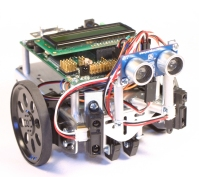
\includegraphics[scale=.5]{img/smallBot}}
\caption{IntelliBrain2 Micro Controller on the standard Ridgesoft base}
\end{figure}\\
This small robot allowed us to learn the basics before moving onto a larger frame.  This robot ran with two independent continuous rotation servos (controlling each wheel independently), a range finding sensor, and two light sensors pointed downwards to help it follow a line.  

Next, we moved onto a larger, faster robot mounted on an Axial Remote Control Rock Crawling car base:
\begin{figure}[h]
\centerline{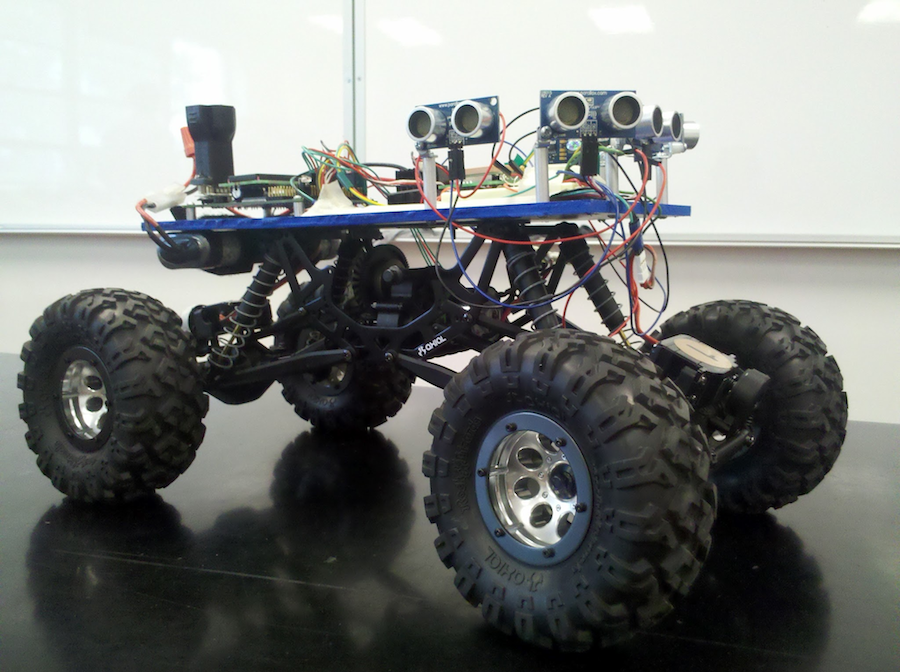
\includegraphics{img/bigBot1}}
\caption{Axial RC car mounted with IntelliBrain2 Controller}
\end{figure}

We modified the base to include 4 wheel steering.  We then mounted a GPS, 5 range finding sensors and a single WheelWatcher Incremental Quadrature Encoder for navigation and speed control.

\subsection{This Documentation}
The purpose of this documentation is to explain the process and steps we took to learn, build, and program our self-navigating robot.  We will introduce the development environment, discuss the specific functions of the robot and describe the running process of the robot, as the end user would see.

\subsection{Project Goals}
\begin{enumerate}
\item Grasp the concepts of introductory robotics.
\item Learn to translate a theoretical environment to a running physical machine.
\item Enhance our understanding of the Java Language.
\item Learn about external Java libraries.
\item Understand how Java can be compiled to a specific platform and handle physical sensor input.
\item Learn advanced robotic algorithms - separate from theoretical Computer Science algorithms.
\end{enumerate}

\clearpage
\section{Development Environment}
The IntelliBrain2 can be programmed in Java.  A specific RoboJDE library is required at compile to interface with the board.  There are numerous options to turn Java code into running code on the robot that we will explain here.
\subsection{Requirements}
First, download the development software from the Ridgesoft Website:\\
{\color{blue}\centerline{http://ridgesoft.com/robojde/robojde.htm}}\\
The software, API, required libraries, and physical wiring diagrams can be found on this website.

There is an included development application, \textit{RoboJDE}, that uses RoboJDE project files $(.rjp)$ to program the robot.  This editor is great for getting started, but is quickly outgrown.  The software comes with many example files and as long as the host computer has a Serial Port (We used an OptiPlex GX620), then there is no additional software required to get the first programs loaded to the robot.

This environment, however, is all plain text with no syntax coloring or error detection.  Moreover, We found Eclipse to be the best editor because it can be configured to automatically compile to the robot using the rsload script.

\subsection{RSLoad Script}
Included in downloads for all platforms is a script called rsload.  rsload is a command line utility for loading code to the robot.  The best documentation on it can be found here:\\
{\color{blue}\centerline{http://ridgesoft.com/robojde/2.0/docs/RoboJDEGuide.pdf}}
Some important arguments to know for rsload are:
\begin{description}

\item[-port] Specifies the port the robot is connected to, typically COM1 on Windows or /dev/ttys0 on Linux, but if using a USB adapter, this could be /dev/tty.usbserial or COM5.  Understanding particular drivers and the OS is important here.
\item[-run] If included, the robot will automatically run when load is complete.
\item[-bank] Specify to load to either Flash or Ram; we always loaded to Flash and in some cases, it was required to use this argument.
\item[-verbose] Good for debugging purposes.
\end{description}

The ultimate required argument is the name of the class that includes main.  An example call:
\begin{verbatim}
rsload -bank Flash -port /dev/tty.usbserial -run Controller
\end{verbatim}
This command will load the Controller class to the robot over the USB to Serial adapter.  When load is complete, it will run the program.  It should be noted that in this example, Controller.class is located in the same directory as rsload.

\subsection{Individual Load Scripts}
For greater compatibility, we wrote a customizable load script that would compile and then load a specific file, given the file path and the name of the file containing the function, $main$.
\small{\begin{verbatim}
#Instructions:
#Update both filePath and fileName variables to represent where the files are.
#These should all be relative to Dropbox.  (Note in eclipse cases, compiled files 
#may be found in the /bin/ directory of the project.  However, these should be 
#pointed to the java file for compiling.
#Don't put a '/' on the end of the filePath:
#The fileName is the main controlling class.
#Warning! Every .java file in the path BETTER compile.
#This is an example:
#filePath=/home/robotics/Dropbox/Robo/Development/Forrest
#fileName=MusicTest
###############################################################
####################### WHAT YOU SHOULD EDIT ####################
filePath=/home/robotics/Dropbox/Robo/Development/Master/Robot/src 
#Note, don't end with /
fileName=Controller		#Note, no .java or .class! This has 'main function'
######################## END WHAT YOU SHOULD EDIT ###############
###############################################################
clear
echo "Welcome to the CS 430 Load Script"
echo "This will fail if RoboJDE is running"
echo ""
echo "Copying to Temp Build Path to not upset Eclipse..."
rm -f /home/robotics/Dropbox/Robo/Development/TempLoadNoTouchie/*
cp $filePath/* /home/robotics/Dropbox/Robo/Development/TempLoadNoTouchie/
echo "Files Copied To Temp Build Path:"
cd /home/robotics/Dropbox/Robo/Development/TempLoadNoTouchie
ls -al
echo "Press Enter to Compile"
read nothing
#Let's compile it first:
echo "Compiling..."
javac -classpath "/home/robotics/RoboJDE/RoboJDE.jar" *.java
echo "Compilation Complete"
echo "Make sure Robot is in Bootstrap Mode, Turn ON then press STOP, 
                                                   Then Press Enter"
read nothing
echo "Initiating Robot Loader:"
sh /home/robotics/RoboJDE/rsload -port /dev/ttyS0 -bank flash $fileName
echo ""
echo "Press Enter to Quit"
read nothing
\end{verbatim}}

This script was written for the robotics user account on an OptiPlex GX620 running Ubuntu 11.10 with the robot connected to the serial port.  It will copy the required files to a temporary directory, compile them and then load them to the robot.

The main purpose of a script like this is to abstract the robot development to simple java files in a single directory.  The script takes care of including the necessary files for interfacing with the board, so the user can write simple Java code to feed this script.

Next, we take this concept one step further by integrating with Eclipse.

\subsection{Integrating with Eclipse}
Eclipse is a robust open source development environment that allows for much customization.  The two requirements for this project are:
\begin{enumerate}
\item Include the RoboJDE.jar archive in the compile path
\item Write an external build tool to automatically call the rsload script.
\end{enumerate}

Once a project is created in Eclipse, preferences can be set by right-clicking on the project root.  Ensure here that the Java Build Path includes the RoboJDE.jar file.  It is convenient to put a copy of this file in the workspace directory so that it can be referenced locally.

There are explicit instructions for setting up an eclipse external tool in the read me, but I have included a screen shot here for further description:
\clearpage
\begin{figure}[h]
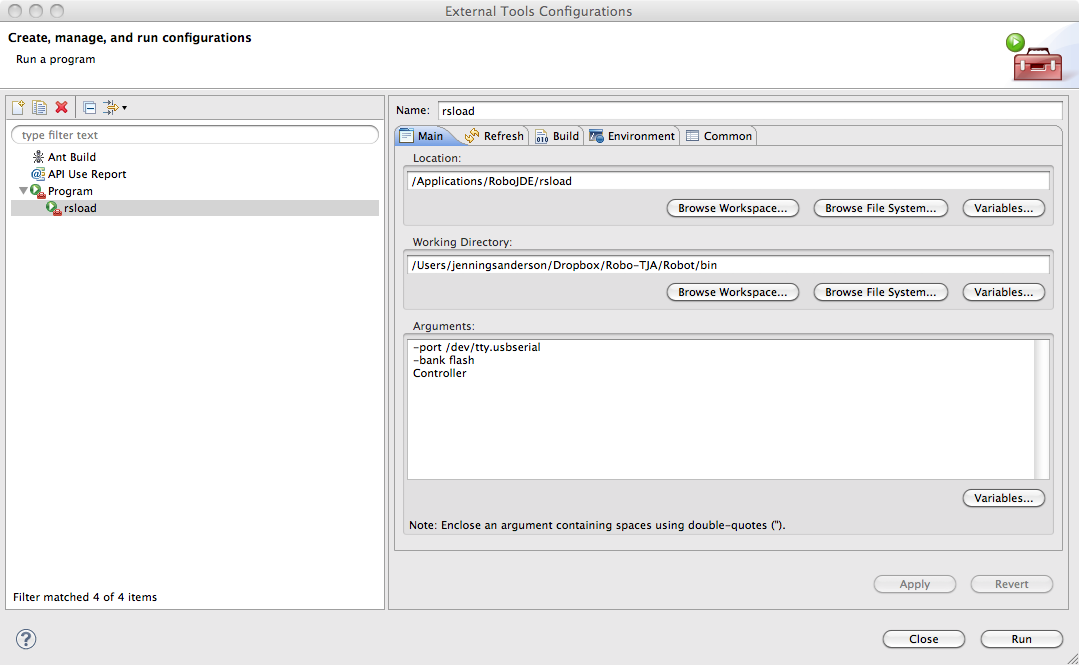
\includegraphics[scale=.4]{img/externalTool}
\caption{Eclipse External Tool Configuration}
\end{figure}

This tool configuration differs from the suggested configuration with static references for convenience.  Note that the Working Directory references the bin directory, where Eclipse puts the compiled class files.  The name of the class with the function, $main$ in it is $Controller$.

\subsection{Source Version Control}
The importance of a steadfast source version control method should not be over looked; unfortunately, we did so for months until turning to git and github.com.  We recommend to spend the time in the beginning familiarizing yourself with the processes of branching, forking, and merging with the github interface.  

We found an open source utility, EGit installed through the Eclipse market place, that allowed us to integrate the Eclipse environment with github.  It should be known and user be warned that github integration with Eclipse is very powerful and will overwrite the local workspace, so one must be comfortable with the github commands and Egit interface before fetching or pushing from the remote repository.

Originally, we used Dropbox, which worked as a great backup tool at the end of the day, but hard for real-time development.  This is because Dropbox is not true version control software.

\subsubsection*{SVC Anecdote on Dropbox}
While Dropbox is a simple, convenient, and magical application in today's computing, it is not a substitute for source version control.  We initially used Dropbox to sync files across all of our computers for team development.  The problem here is that changes propagate immediately.  Backups are kept in the depths of Dropbox's servers, but are tedious to scan through and recover.  However, the real kicker occurs when Dropbox meets DeepFreeze, the Enterprise software that Carroll uses to fight malicious intentions.  If Dropbox is installed on a user's profile, it will by default sync all files to a folder on the local hard drive.  When the computer restarts, changes to the $C$ drive are erased and Dropbox is fooled into believing the user deleted all files in their Dropbox directory.  This change is then propagated to the rest of the team, so come Monday morning, all code is erased across every team member's computer.  \textit{Thanks, Forrest}.

\clearpage
\section{Physical Robot Design}
Here we describe the physical attributes of the robot, after introducing each part, the next section will cover the logic that governs each physical interface.
\begin{figure}[h]
\centerline{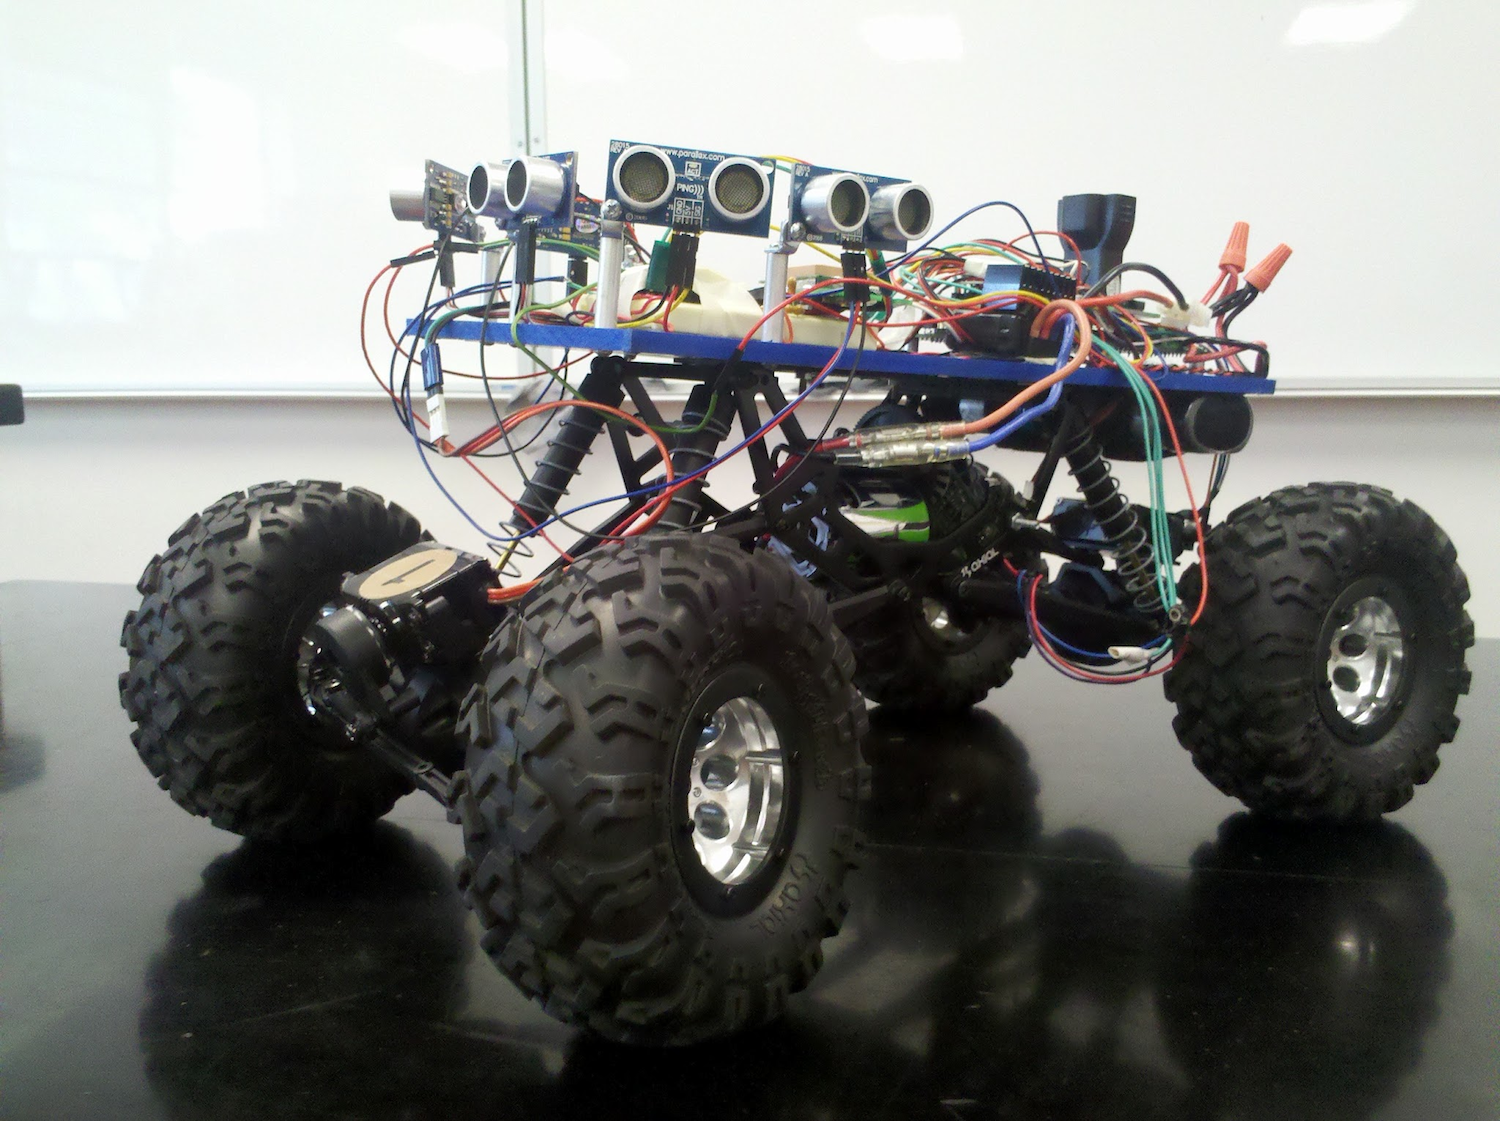
\includegraphics[scale=.75]{img/bigBot2}}
\caption{Final Robot Design}
\end{figure}
\subsection{Description}
The Robot is about 18" long, 10" tall, and 11" wide.  It has 4 wheels of 5" diameter. and runs off a 3000 mAh Ni-MH battery.  The RC car body is designed by Axial Racing ({\color{blue} www.axialracing.com}).

Borrowing the parts from a second RC car, we gave our robot 4-wheel steering by substituting the rear axle with a second car's front steering axle.
\begin{figure}[h]
\centering
\subfloat[Front Steering]{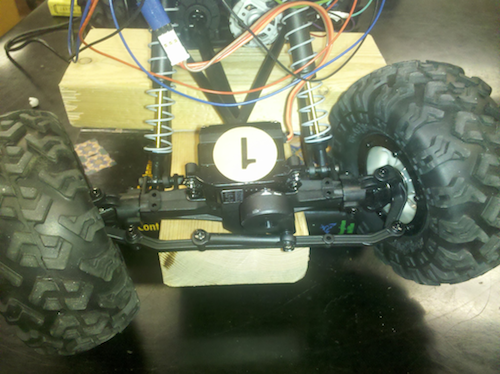
\includegraphics{img/steering1}}
\hspace{5mm}
\subfloat[Rear Steering]{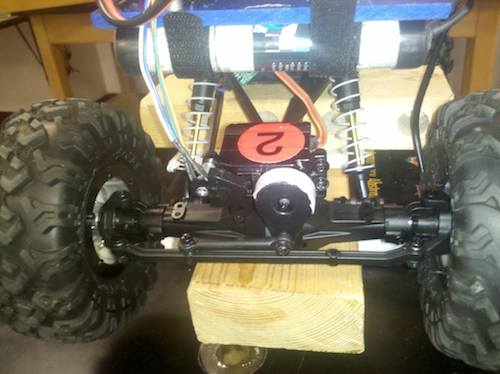
\includegraphics{img/steering2}}
\end{figure}

A central motor, controlled by an Axial AE-2 ESC drives all four wheels.  This is mounted in the center of the body and is directly linked to the WheelWatcher chip which records how fast the motor is spinning.
\begin{figure}[h]
\centerline{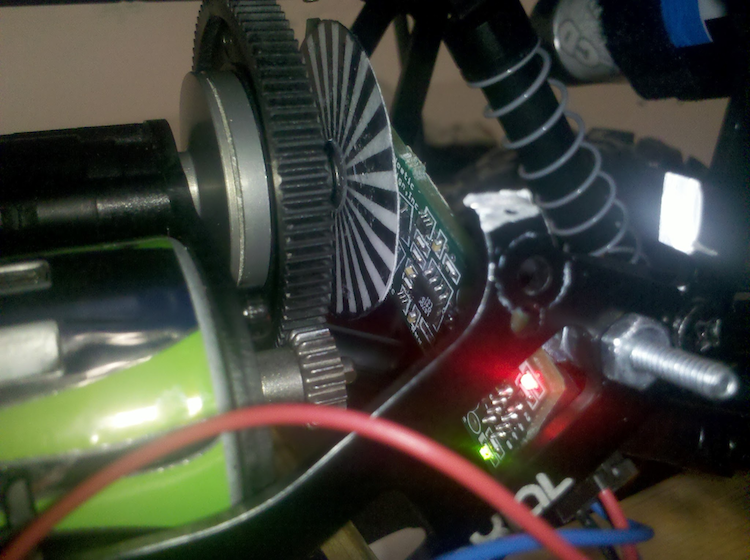
\includegraphics{img/wheelwatcher}}
\caption{Nubotics' WheelWatcher Incremental Quadrature Encoder mounted next to motor}
\end{figure}

As the motor turns, the black and white disk spins over light sensors on the WheelWatcher chip.  With each change in color, a counter is incremented.  This counter can then be converted to rotations per minute, or $RPM$.

On the top of the robot are 5 range finding sensors that operate by sonar:
\begin{figure}[h]
\centerline{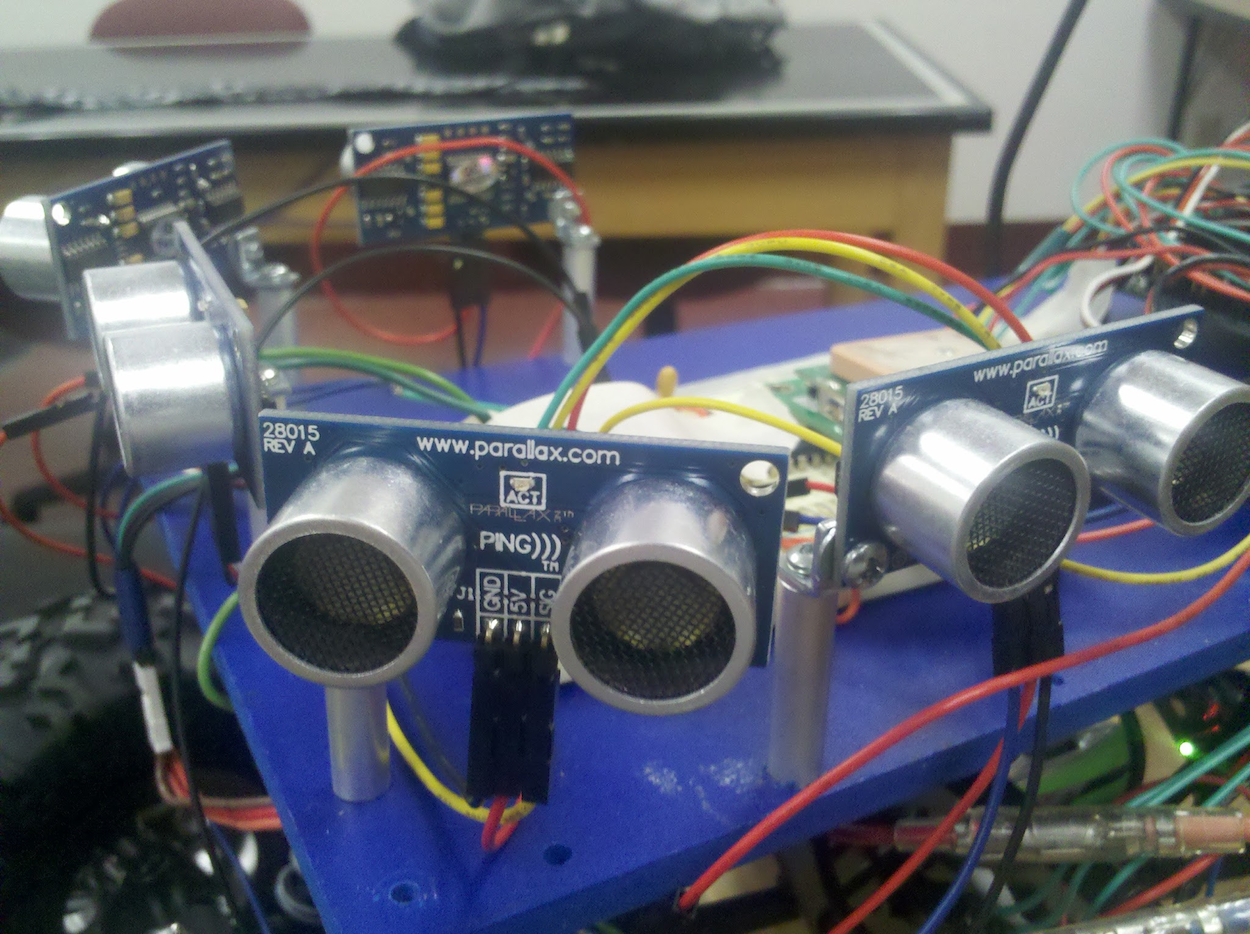
\includegraphics[scale=.8]{img/rangeSensors}}
\caption{Ping))) Sensors}
\end{figure}

These 5 sensors point directly ahead, 45\textdegree \hspace{1mm}left, right, and 90\textdegree \hspace{1mm}left, right.  They operate via sonar and require special attention to timing as the command tells it when to send a `ping' and when to read the ping.  If not a enough or too much time elapses between the send and read command, the data is corrupted.

Ultimately, the main controlling board is the IntelliBrain2 by Ridgesoft: 
\begin{figure}[h]
\centerline{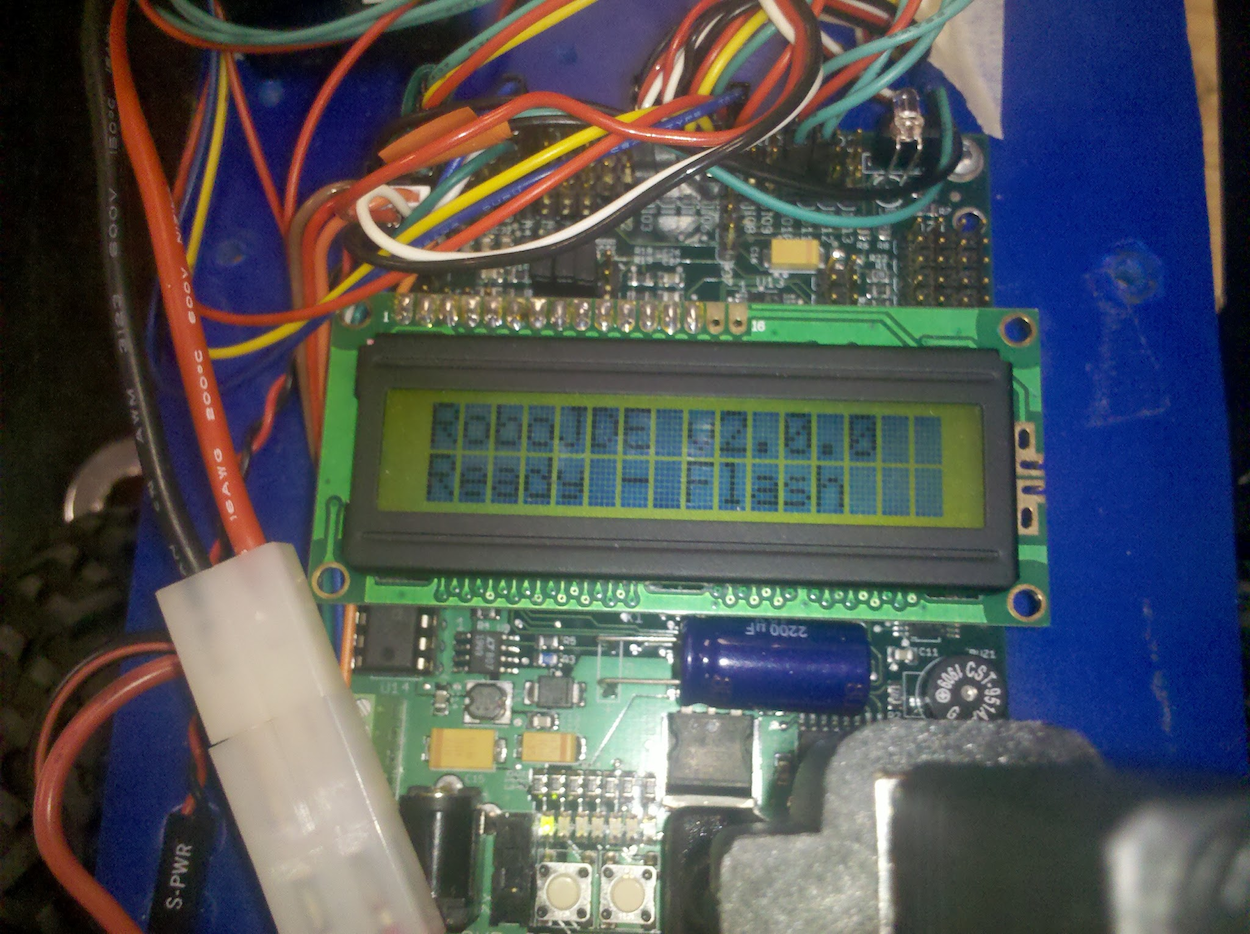
\includegraphics{img/intellibrain}}
\caption{The 14.7 MHz IntelliBrain2 MicroController}
\end{figure}

This is a Java programmable board that calls a specific API to interface with the physical inputs.  It connects to a computer via a serial port.  In this figure, we have a USB adapter plugged into the serial port. 


\clearpage
\section{Robot Logic}
There are 2 main obstacles that we overcame in this project:
\begin{enumerate}
\item Difference between Theory and Application
\item CPU Clock Speed
\end{enumerate}
The difference between theory and application deals with the inconsistencies in a physical environment.  On the white board and in the computer, issuing commands such as \textit{turnRight(35\textdegree)} then \textit{goForward(10 inches)} would move the robot 10 inches at 35\textdegree from the current location.  

In a physical environment, this is never the case, especially when working with a remote control vehicle.  The driving surface may be inconsistent, making the wheels only turn 30\textdegree and the battery may be low, so the motor may not drive at the proper speed, making the car only go 9 inches.  A series of this mistakes and the robot will lose its heading completely.  

Similarly, if a range finding sensor misfires and returns false data, decision making processes are misinformed.  On the white board, a command such as \textit{getDistance()} can be trusted, but in reality, these functions must be checked and double checked for errors before they can be trusted by the robot.
\vspace{2mm}

In previous Computer Science courses, we were never limited by the speed of the CPU.  Sure it may take time to compute \textit{factorial(16984)}, but the impact of this time has never had high consequences.

For this robot, we have become very aware of exactly how long it takes the CPU to complete a cycle.  This has two ramifications:
\begin{enumerate}
\item How long will a set of commands tie up the CPU? \textit{If it takes too long to interpret sensor data, then the robot may hit the wall before it realizes the wall is there.}
\item How fast is the CPU? \textit{If a particular sensor is running substantially faster than the CPU, can the robot even interpret that data?}\footnote{See the section on Remote Control}
\end{enumerate}

\vspace{2mm}
We have to consistently work to overcome the difference between theory and application in robotics, but seem to have worked out a few tricks to function thus far.  In terms of physical CPU limitations, we separated sensors and logic into various threads with specific priorities.

\clearpage
\subsection{Threads}
The IntelliBrain2 MicroController has the ability to spawn multiple process threads.  As such, we have separated our robots sensory inputs and logic into different threads to optimize driving abilities.  These threads (in order of priority) are:

\begin{quote}
\begin{description}
\item[Remote] Handles checking for the remote to turn on (wireless kill switch)
\item[Sonar] Controls the 5 range finding sensors on the front.
\item[Brain] Governs all decision making
\item[Engine] Controls the motor servo.
\item[Steering] Controls the front and rear steering servos.
\item[GPS] Controls the Global Positioning System chip that is mounted on the top of the robot.
\item[Debugging] Handles debugging data if requested - has minimum priority.
\end{description}
\end{quote}

This design is based off the general principle of ranking importance as: \textit{1) Sensory Input 2) Decision-Making 3) Motor Control}  (Note, the GPS is excluded in this because it is rarely used).

\subsubsection{Challenges}

\clearpage
\subsection{Sonar \& Range Finding}
The Robot has 5 range finding sensors that operate via sonar.  That is, they emit a sound wave and measure the time it takes for the wave deflect off an object and return.  Since the speed of sound is constant, the distance it traveled in the measured time can be determined.  In order to get 5 sensors active, a relay had to be added to the circuit to overload the digital input ports on the IntelliBrain2.

	As a result, when sonar is running, there is a ticking noise as the relay switches back and forth.  The logical obstacles we overcame with the sonar sensors was timing.  There is a window of time between when the sensor has received the signal and the sensor trashes the signal.  If you ask for the distance too soon after telling the sensor to \textit{ping()} (emit a sound wave), there will be no data to receive.  Too long and the data is no longer valid or trashed by the sensor.

Here is a diagram of the sensor we used and its function:\footnote{Image from http://www.generationrobots.com/site/medias/Principe-fonctionnement-Sonar-Ping-Parallax.JPG}

\begin{figure}[h]
\centerline{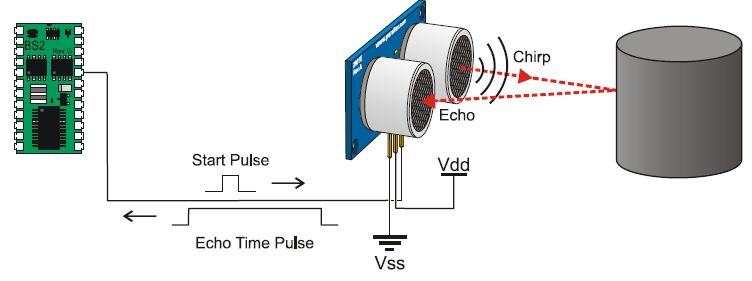
\includegraphics[scale=.8]{img/sonar}}
\caption{Parallax Ping))) Sensor}
\end{figure}

The timing issue made us shy away from using Threads at first because we could not control the timing very accurately if the processor was determining which processes got to run when; however, we ultimately decided to run the sensors iteratively as a single thread with hard coded 200 millisecond delays between thg ping and the retrieval of information from the sensor.

The two side sensors (East and West) are connected to the relay and take turns as active distance sensors.

\clearpage
\subsection{Engine \& Motor}
One of the more difficult parts of the robot to program, the motor, an Axial 27T electric motor is controlled by the Axial AE-1 ESC.  These are the two parts:\footnote{Images from: http://axialracing.com/ftp/ax10rtr/}

\begin{figure}[h]
\centering
\subfloat[27T Electronic Motor]{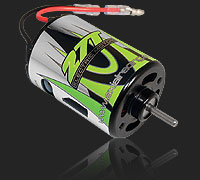
\includegraphics[scale=.85]{img/motor}}
\hspace{5mm}
\subfloat[Axial AE-1 ESC]{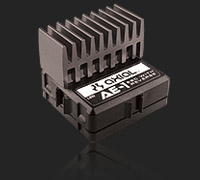
\includegraphics[scale=.85]{img/ae1}}
\end{figure}

The AE-1 is connected to one of the MicroController's servo ports and we initialize it as a \textit{continuous rotation servo}.  This means that it takes integer arguments for the command \textit{setPower(int n)} between -16 and 16 (negative numbers representing reverse).  

Additionally, active braking is available, so if the controller gets a command for the opposite direction, it will brake and bring the motor to a stop.

The motor control is the ultimate showcase of theoretical versus physical programming.  The values passed to \textit{setPower()} never represent the same speed.  There are too many factors: battery level, how long its been running, what speed it was going, driving surface, etc.

To remedy this, we wrote a separate driver called Engine that uses the Nubotic Wheel Watcher chip\footnote{Image in previous section} to count the rotations of the motor.  This is calculated to the number of rotations-per-minute (RPM) so that we can receive active feedback on the current wheel speed.

From here, we can attempt the general motor control logic:
\begin{enumerate}
\item Set a desired velocity; if not 0, set the motor power to a specific range that somewhat corresponds to that velocity.
\item Get the current RPM of the motor
\item If the RPMs are  higher than desired, decrease motor power.
\item If the RPMS are too low, increase motor power if its not already at maximum level.
\item Go To Step 2.
\end{enumerate}

To implement this motor logic, we used a proportional-integral-derivative (PID) Controller.

The PID is the most commonly used feedback controller.  It works to minimize error by adjusting input variables:\footnote{Image and Description from Wikipedia: http://en.wikipedia.org/wiki/PID\_controller}
\begin{figure}[h]
\centerline{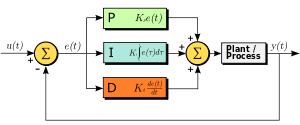
\includegraphics{img/PID}}
\caption{PID Controller Diagram}
\end{figure}

The PID controller is initiated in the Engine class and then motor power is set based on feedback from the PID given the inputs: \textit{desired rpm, actual rpm}.  Using the PID controller helped cut down on 'juttiness' of the robots movements.

\clearpage
\subsection{Wheels \& Steering}
The two steering servos (front and back) are attached to separate servo ports on the Micro Controller.  These are initiliazed as standard servos and as such can take the argument \textit{setPosition(int n)} where $n$ is an integer between 0 and 100, 50 being the midpoint.

The rear servo is set to the value: 100-(value of front servo).

\subsubsection*{Steering Servo Challenges}
When the robot first turns on, the steering range must be reset.  We found that the best way to do this is to perform a small calibration by turning the wheels all the way one direction and then all the way to the other direction then back to the middle (50).  After this, the 0-100 range for the servo method, \textit{setPosition(int n)} gives full range of motion for the wheels.

If this is not done properly, then the steering range is incomplete and inconsistent.  We attempted putting a sensor on the steering servo to check the wheels were at the appropriate spot, but found consistency after this calibration routine.
\vspace{2mm}
Additionally, the original steering mechanism was built to allow the wheels to slip dramatically - this was a feature of this particular Remote Control vehicle that was made for crawling over rocks.  This slip lead to major complications in robot control because the logic had no way to tell if the wheels were pointing the direction the servo said they were.\footnote{Provided the servo was in the position it claimed to be! (Before calibration)}

To overcome this, we padded the slipping mechanism with paper towel to absorb the play.  This seems to fix all the complications.  However, now if the robot hits a wall or bumps the wheel too hard, the steering shaft and the steering motor take the brunt of the force, so one must be more careful in operating the robot.


\clearpage
\subsection{Remote Control}
In a major addition to the robot, we incorporated the original RC car remote to override the robot logic for motor control.  This was done to serve two purposes: 1) act as a kill switch and 2) provide the ability to manually drive the robot to train a Neural Network.  We played with this idea early on, but abandoned it due to difficulty in obtaining clean data from the remote.

Upon revisiting the idea, we determined the original problem was a limitation in the physical clock speed of the Micro Controller.  The IntelliBrain2 has a clock speed of 14.7 MHz.  The frequency of the remote is 27 MHz.  Therefore, no matter how many consecutive clock cycles we gave the remote sensor, it was incapable of accurately sampling the change in signal.

To remedy this issue, our team member pursuing a Physics degree created an RC circuit (a type of Low-Pass filter) for the remote sensor that cleaned up the signal and allows for meaningful sampling of the analog input.  
\begin{figure}[h]
\centerline{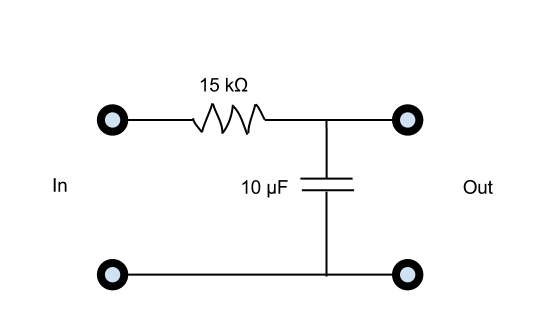
\includegraphics[scale=.5]{img/circuit}}
\caption{Nate's Low-Pass Filter Circuit Diagram}
\end{figure}

We should note that this current circuit is an improvement on the first attempt which utilized much larger capacitors that \textit{featured} a multiple second delay on steering and throttle input.

\subsubsection*{Remote Input}
After averaging the 3 sample points (for consistency), we can obtain nearly real-time steering and throttle input.  Because we must wait for the capacitor to charge/discharge, there is some lag in control.\footnote{After all this, we've succeeded in building a simple RC car (worse than the one we started with)}

The impact of this feature is a physical kill switch: Turn the remote on and the running logic stops and the remote takes over.\footnote{Also, the \textit{Mario} theme song plays}; turn off the remote, and the running logic resumes.


\clearpage
\subsection{Neural Network}
{\color{red} Going to need Nate's help on this part...}

\clearpage
\subsection{Global Positioning System}
The robot does include a GPS chip on the body that interfaces with the board.  This allows it to track is position via satellites.  Currently, we do not incorporate this data into our logic, but the interface and control exist.

\clearpage
\subsection{Debugging}
The robot initializes a separate thread with minimum priority dedicated to debugging.  It takes input from the thumb wheel and STOP/START buttons to interface with the user and print running information to the LCD Display on the MicroController.

Options for debugging are as follows:
\begin{quote}
\begin{enumerate}
\item Sonar Debug
\item Steering Debug
\item Engine Debug
\item Remote Debug
\end{enumerate}
\end{quote}





\clearpage
\section{Robot User Manual}
\subsection{Starting Out}
The battery attaches via Velcro straps under the back of the robot.  It plugs into both the motor and the MicroController.  Once the battery is connected, the robot can be turned on by the on/off switch on the MicroController.
\vspace{2mm}
Just press the START button to start the robot.  A small calibration routine will automatically run as the robot shifts the wheels back and forth.

\subsection{Interacting with the Robot}

\clearpage
\section{Conclusion}
This project was quite the crash course in Robotics.  It seemed to incorporate aspects from every Computer Science course we've taken over the years: Finite States, Process Scheduling, Physics, Algorithm design, and more.


\subsection{Strengths}
\subsection{Weaknesses}

\clearpage
\section{Appendix}
The following pages include most of the source code for the robot.
\subsection{Source Code}

\end{document}